\chapter[Turbulencia]{Breve introducción a la turbulencia}\label{Turbulencia}
\section{Promediado de Reynolds}

	
	\begin{itemize}
		\item Los flujos que encontramos en la industria, en el laboratorio, en
		la naturaleza son, normalmente, turbulentos.
		
		\begin{itemize}
			\item Excepciones: lubricación, microfluidos, \ldots{}
		\end{itemize}
		\item La \textcolor{blue}{transición a la turbulencia} ocurre para un determinado
		número de Reynolds, que no tiene porqué ser muy alto. Este \textcolor{red}{número
			de Reynolds crítico} depende del fenómeno en particular. 
		
		\begin{itemize}
			\item Por ejemplo, para flujo alrededor de una esfera, el flujo empieza
			a mostrarse turbulento para Re $\approx3\times10^{5}$. En el caso
			de flujos en el interior de una tubería, la transición puede empezar
			incluso para Re $\approx2000$, en función de las características.
		\end{itemize}
		\item Un flujo turbulento esta caracterizado por 
		
		\begin{itemize}
			\item la \textcolor{red}{imprevisibilidad}
			\item el \textcolor{red}{desorden} y 
			\item las rápidas \textcolor{red}{fluctuaciones}. 
		\end{itemize}
	\end{itemize}

	
	En teoría, debería ser posible su estudio con las ecuaciones de la
	dinámica ya estudiadas, pero, como se comentó anteriormente, estas
	ecuaciones son no-lineales, y tan solo se pueden resolver de forma
	analítica en muy pocos casos.
	
	Una solución es la resolución numérica. Pero esto implica un problema:
	
	Para poder resolver numéricamente las ecuaciones de Navier-Stokes,
	antes hay que discretizar el dominio de estudio, creando una malla.
	

\begin{center}
	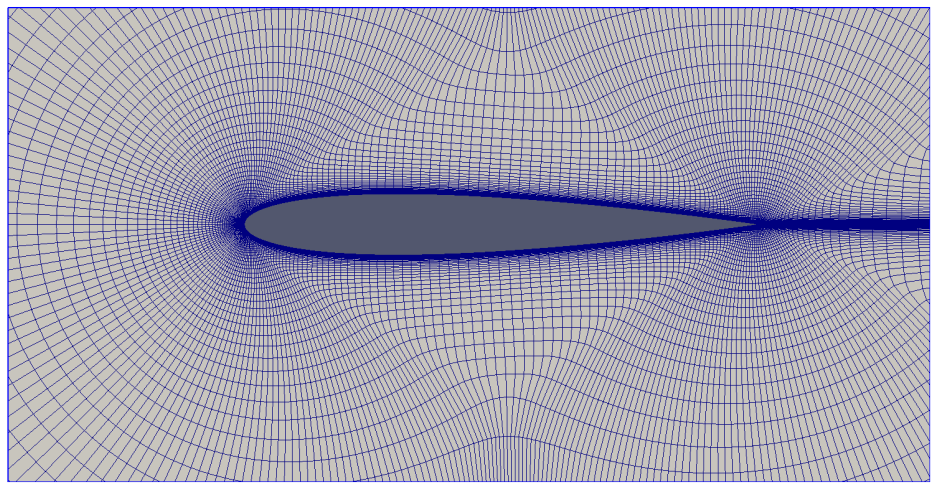
\includegraphics[width=0.7\linewidth]{TeX_files/chapter07-Turbulencia/airfoil}
\end{center}
	
	
	\begin{itemize}
		\item Las fluctuaciones espaciales de flujo turbulento son de varias escalas.
		Cuanto mayor es Re, más pequeñas pueden llegar a ser las fluctuaciones,
		y más fina tiene que ser la malla. 
		\item Pero, por otro lado, la resolución de la malla está limitada por la
		potencia del ordenador que se utilice. De este modo, el hardware nos
		limita Re.
		\item La potencia de los superordenadores crece de forma espectacular (ley
		de Moore), y el número de Reynolds de las simulaciones directas de
		las ecuaciones de Navier-Stokes va creciendo. Pero no todo el mundo
		tiene acceso a ellos.
		\item Cuando no es posible resolver de forma directa las ecuaciones de Navier-Stokes
		debido a que Re es muy grande y, por lo tanto, tendríamos que llegar
		a fluctuaciones de muy pequeño tamaño, se recurre a modelos de turbulencia,
		que nos predicen el comportamiento de las pequeñas escalas, de forma
		que sólo tenemos que preocuparnos de simular las grandes.
	\end{itemize}
	
	\textbf{Idea fundamental :}
		magnitud = magnitud media + fluctuaciones de magnitud.

	P.e., cualquier componente de la velocidad, o la presión : 
	\[
	u=\mean{u}+u'\,;\,p=\mean{p}+p'
	\]
	
	
	Consideremos que $L$ es una distacia típica macroscópica de nuestro
	problema (podría ser el tamaño medio de la discretización que nos
	podemos permitir con nuestro ordenador).
	
			
			\begin{center}
				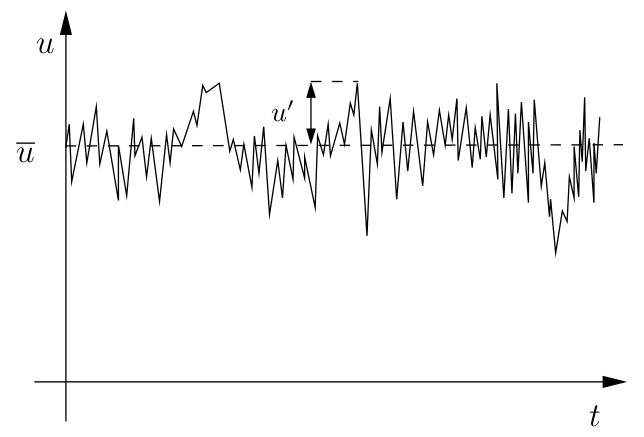
\includegraphics[width=0.7\linewidth]{TeX_files/chapter07-Turbulencia/noise}
			\end{center}
			

				\[
				\mean{u}=\frac{1}{T}\int_{0}^{T}u \dif t
				\]
				
				\[
				u'(x)=u-\mean{u}
				\]
				
				\[
	\mean{u'}=\mean{u-\mean{u}} =\mean{u}-\mean{\mean{u}}=\mean{u}-\mean{u}=0
				\]
			
			
			
				\[
				\mean{u'^{2}}=\frac{1}{T}\int_{0}^{T}u'^{2}\dif t\neq0
				\]
			

	
	La \textcolor{red}{intensidad de la turbulencia} se define como $I=\frac{\sqrt{\mean{u'^{2}}}}{\mean{u}}$
	
	Por regla general, $I$ en flujos típicos en Ingenieria es del orden
	del 10\% o 20\%.
	
	El producto de promedios no es necesariamente nulo. 
	\begin{align*}
		\mean{u'v'} & \neq0\\
		\mean{u'p'} & \neq0
	\end{align*}
	
	
	Descomponemos en promedios y fluctuaciones las tres componentes de
	la velocidad, 
	\begin{eqnarray*}
		u & = & \mean{u}+u'\\
		v & = & \mean{v}+v'\\
		w & = & \mean{w}+w'
	\end{eqnarray*}
	y escribimos la ecuación de continuidad para fluido incompresible
	\[
	\dparc{u}{x}+\dparc{v}{y}+\dparc{w}{z}=0
	\]
	usando esta descomposición 
	\[
	\dparc{}{x}\left(\mean{u}+u'\right)+\dparc{}{y}\left(\mean{v}+v'\right)+\dparc{}{z}\left(\mean{w}+w'\right)=0\;\Rightarrow\;\vec{\nabla}\cdot\vec{u}+\vec{\nabla}\cdot\vec{u}'=0
	\]
	
	
	Realizamos un promedio sobre esta expresión, 
	\[
	\mean{\vec{\nabla}\cdot\vec{u}}+\mean{\vec{\nabla}\cdot\vec{u}'}=\vec{\nabla}\cdot\mean{\vec{u}}+\underbrace{\vec{\nabla}\cdot\mean{\vec{u}'}}_{=0}=0.
	\]
	
	Esto indica que tanto la velocidad promedio como la fluctuación deben
	cumplir la condición de continuidad.
	
	\begin{eqnarray*}
		\vec{\nabla}\cdot\mean{\vec{u}} & = & 0\\
		\vec{\nabla}\cdot\vec{u}' & = & 0
	\end{eqnarray*}
	
	Escribimos también las ecuaciones de NS con esta descomposición y,
	a continuación, las promediamos. 
	
	Esto es lo que se conoce como \textbf{\textcolor{red}{Ecuaciones de
			Navier Stokes con Promediado de Reynolds}} (en inglés, RANS, Reynolds
	Averaged Navier Stokes). 

	
	Consideremos, por simplicidad, únicamente el caso de la componente
	$x$: 
	\[
	\rho\left[\dparc{u}{t}+u\dparc{u}{x}+v\dparc{u}{y}+v\dparc{u}{y}\right]=-\dparc{p}{x}+\dparc{\tau_{xx}}{x}+\dparc{\tau_{xy}}{y}+\dparc{\tau_{xz}}{z}
	\]
	donde el tensor de tensiones es sin traza, incluida en el término
	de las presiones.
	
	El primer término, después de promediar queda 
	\[
	\rho\dparc{\mean{u}}{t},
	\]
	igual que el término del gradiente de presión 
	\[
	\dparc{\mean{p}}{x}.
	\]
	
	
	En cambio, en la aceleración convectiva aparecen unos términos extras,
	\begin{eqnarray*}
		\mean{u\dparc{u}{x}}=\mean{u}\dparc{\mean{u}}{x}+\mean{u'\dparc{u'}{x}}=\mean{u}\dparc{\mean{u}}{x}+\dparc{}{x}{\mean{u'u'}}-\mean{u'\dparc{u'}{x}}\\
		\mean{v\dparc{u}{y}}=\mean{v}\dparc{\mean{u}}{y}+\mean{v'\dparc{u'}{y}}=\mean{v}\dparc{\mean{u}}{y}+\dparc{}{y}{\mean{v'u'}}-\mean{u'\dparc{v'}{y}}\\
		\mean{w\dparc{u}{z}}=\mean{w}\dparc{\mean{u}}{z}+\mean{w'\dparc{u'}{z}}=\mean{w}\dparc{\mean{u}}{z}+\dparc{}{z}{\mean{w'u'}}-\mean{u'\dparc{w'}{z}}
	\end{eqnarray*}
	
	\subsection*{Actividad 1:}
		Deducir las expresiones anteriores

\bigskip
	
	La ecuación de NS se puede escribir, después de reordenar términos,
	como
	
	\[
	\boxed{{\begin{split}\rho\left[\dparc{\mean{u}}{t}+\mean{u}\dparc{\mean{u}}{x}+\mean{v}\dparc{\mean{u}}{y}+\mean{w}\dparc{\mean{u}}{z}\right]=\\
				-\dparc{\mean{p}}{x}+\dparc{}{x}\bigl(\tau_{xx}-\rho\mean{u'u'}\bigr)+\dparc{}{y}\bigl(\tau_{xy}-\rho\mean{v'u'}\bigr)+\dparc{}{z}\bigl(\tau_{xz}-\rho\mean{w'u'}\bigr)
			\end{split}
	}}
	\]
	
	dado que 
	\[
	\mean{u'\dparc{u'}{x}}+\mean{u'\dparc{v'}{y}}+\mean{u'\dparc{w'}{z}}=\mean{u'\underbrace{\left(\dparc{u'}{x}+\dparc{v'}{y}+\dparc{w'}{z}\right)}_{=0}}=0
	\]
	

\section{Interpretación física del tensor de Reynolds}

	
	\begin{itemize}
		\item Las ecuaciones de Navier-Stokes para las velocidades y presión promedios
		son idénticas, excepto por la aparición de unos términos $-\rho\mean{u_{i}'u_{j}'}$,
		que se comportan como unos esfuerzos.
		\item Estos esfuerzo son los debidos a la cantidad de movimiento turbulenta
		transportada en el flujo, y son los responsables de la disipación
		de energia debida a las fluctuaciones.
		\item Estos términos $-\rho\mean{u_{i}'u_{j}'}$ forman el \textcolor{red}{tensor
			de esfuerzos turbulento}, o \textcolor{red}{tensor de Reynolds}. 
		\[
		\tau_{ij}^{t}=-\rho\mean{u_{i}'u_{j}'}
		\]
	\end{itemize}

	
	Nadie sabe a ciencia cierta cómo es este tensor, pero Prandtl propuso
	en 1930 el concepto de \textcolor{red}{viscosidad turbulenta}, $\mu_{t}$,
	como analogia con la viscosidad molecular y la ley de viscosidad de
	Newton, 
	\[
	\tau_{ij}^{t}\approx\mu_{t}\dparc{\mean{u_{i}}}{x_{j}}.
	\]
	Pero de nuevo nos encontramos con el problema del valor de $\mu_{t}$.
	Existen muchos modelos para calcularla, y el más sencillo fue propuesto
	también por Prandtl, y es conocido como el \textcolor{red}{modelo
		de la longitud de mezcla}, 
	\[
	\mu_{t}\approx\rho l^{2}\left|\dparc{\mean{u_{i}}}{x_{j}}\right|
	\]
	
	La longitud de mezcla $l$ es algo equivalente al recorrido libre
	medio de las partículas de un gas en mecánica estadística. Su valor
	dependerá del problema en concreto que queramos resolver.

\section{Ley de pared y capa límite turbulenta}

	
	El estudio de casos generales de flujos turbulentos es extremadamente
	complicado. Un caso relativamente sencillo es el estudio del flujo
	cerca de un sólido. Esta zona, en la que la velocidad del fluido tiende
	de forma suave a la del sólido es conocida como \textcolor{red}{capa
		límite}. Aquí tan sólo vamos a estudiarla de forma superficial, dejando
	este importante tema para más adelante.
	
\begin{center}
	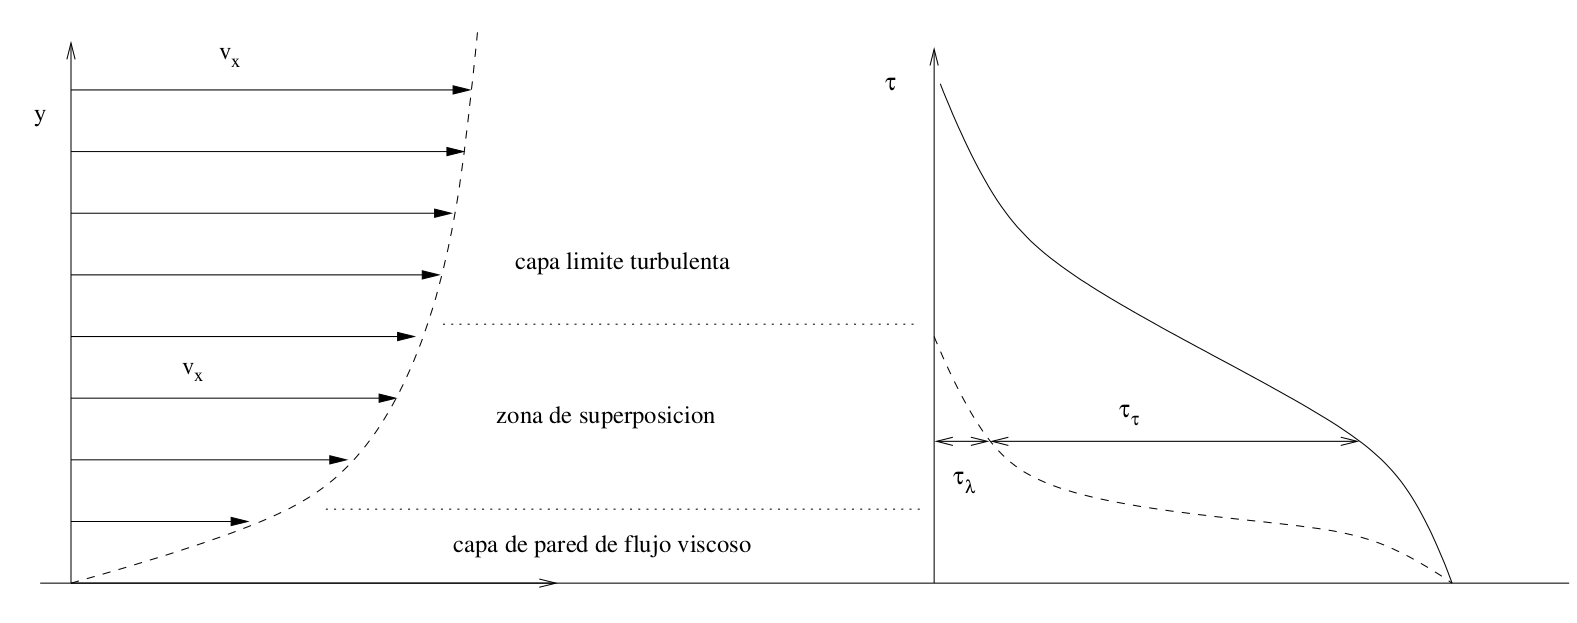
\includegraphics[width=0.7\linewidth]{TeX_files/chapter07-Turbulencia/pared}
\end{center}

	
	\begin{itemize}
		\item El espesor de la capa límite se define como la coordenada $y$ para
		la cual la velocidad alcanza el 99\% de la velocidad que tiene asintóticamente
		para $y\rightarrow\infty$. 
		\item $\tau_{p}$ es el esfuerzo tangencial en la pared.
		\item En la zona de la capa de pared, el flujo es laminar ya que la velocidad
		es pequeña y la viscosidad domina. 
		\item En esta zona, Prandtl dedujo en 1930 que el perfil de velocidad no
		puede depender del espesor de la capa límite, $\delta$. 
		\[
		u=f(\mu,\tau_{p},\rho,y)
		\]

		\item Por análisis dimensional, sabemos que esta ley estará definida por
		2 grupos adimensionales. 
		\[
		u^{+}=F(y^{+})
		\]
		donde 
		\[
		u^{+}=\frac{u}{u^{*}}\,;\,y^{+}=\frac{\rho u^{*}y}{\mu}\,;\,u^{*}=\sqrt{\frac{\tau_{p}}{\rho}}
		\]
		\item $u^{*}$ se denomina \textcolor{red}{velocidad de fricción} y, aunque
		tiene unidades de velocidad, en realidad no lo es.
		\item A la expresión $u^{+}=F(y^{+})$ se conoce como \textcolor{red}{ley
			de pared}, y llega hasta $y^{+}\approx10$. 
		
		\begin{itemize}
			\item Esta ley puede ser, por ejemplo, lineal, $u^{+}=y^{+}$.
		\end{itemize}
	\end{itemize}

	
	En cuanto a la capa externa turbulenta, el mismo Prandtl en 1933 dedujo
	que, dado que es turbulenta, la viscosidad no es importante, y la
	diferencia de la velocidad respecto de ${u}_{\infty}$ es función
	únicamente de $y$, del espesor de la capa límite, $\delta$, del
	esfuerzo tangencial en la pared, $\tau_{p}$, y de la densidad $\rho$,
	${u}_{\infty}-u=g(\delta,\tau_{p},\rho,y)$. De nuevo, el teorema
	$\Pi$ de Buckingham nos indica que esta ley viene dada por dos grupos
	adimensionales, 
	\[
	\frac{{u}_{\infty}-u}{u^{*}}=G\left(\frac{y}{\delta}\right).
	\]
	
	En la zona intermedia, sean cuales sean las formas de $F$ y $G$,
	éstas deben superponerse de forma suave. Se puede demostrar que ésto
	es sólo posible si la ley de velocidades en esta zona es logarítmica.
	\[
	\boxed{\frac{u}{u^{*}}=\frac{1}{\kappa}\ln\frac{\rho u^{*}y}{\mu}+B}
	\]
	con $\kappa\approx0.41$ y $B\approx5.0$. Ésta es la \textcolor{red}{ley
		logarítmica de superposición}, y se extiende hasta $y^{+}\approx1000$

	
	Del Kundu\cite{Kundu2012} (figura 12.18):
	
\begin{center}
	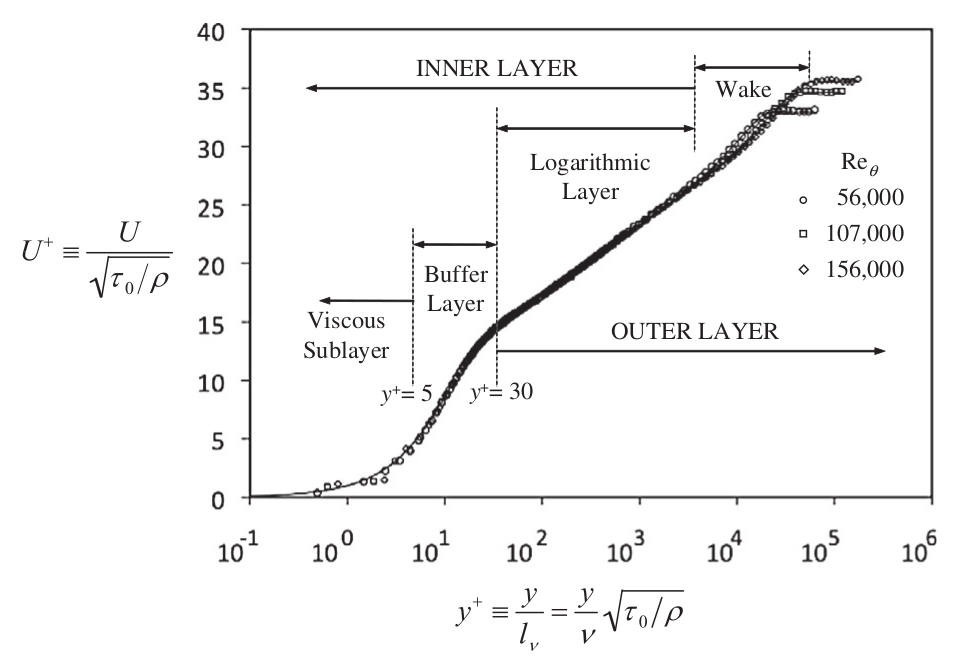
\includegraphics[width=0.7\linewidth]{TeX_files/chapter07-Turbulencia/LawOfWall}
\end{center}


	
	\subsection*{Actividad 2:}
		Si se considera el modelo de longitud de mezcla de Prandtl, cerca
		de la pared, con $l=\kappa y$, ($\kappa=0.41$ es la constante de
		Prandtl), se puede obtener la ley logarítmica de superposición, considerando
		que la ley de pared es lineal, $u^{+}=y^{+}$+ hasta $y^{+}=10$.
		
		Pista: considerar que $\tau_{t}\approx\tau_{p}$ independientemente
		de $y$.

	\subsection*{Actividad 3:}
		Para agua a 10 m/s de velocidad máxima, entre dos placas separadas
		1 cm, suponiendo que el flujo sigue la ley logarítmica, calcular $\tau_{p}$
		y el espesor de la subcapa laminar. Compara con el valor obtenido
		de $\tau_{p}$ si hubiesemos supuesto un flujo laminar viscoso, 
		\[
		u=\frac{4u_{max}}{h^{2}}y(h-y)
		\]

